\chapter{Solution à symétrie sphérique et métrique de Schwarzschild}

    \section{Solution de Schwarzschild}
    
        Cherchons à résoudre les équation d'Einstein
        \begin{equation}
            R_{\mu\nu}-\frac{1}{2}Rg_{\mu\nu} = 8\pi G T_{\mu\nu}
        \end{equation}
        avec $R_{\mu\nu} = 0$ dans le vide. Cette égalité tensorielle est équivalente à $10$ équations linéaires aux dérivées partielles. Cependant, les $4$ égalités de Bianchi sont contenue dans la condition $\nabla_\mu G^{\mu\nu}$ qui est automatiquement satisfaite. Il n'y a en fait que $6$ équations. Les inconnues de ces équations sur les composantes de $g$. Le tenseur métrique possède $10$ composantes indépendantes mais $4$ de ces composantes sont des fonctions arbitraire provenant d'un changement de coordonnées $x'(x)$. Il n'y a donc réellement que $6$ inconnues, pour $6$ équations.\\
        
        Pour trouver des solutions, on peut essayer d'imposer des contraintes de symétrie au champ de gravitation, c'est-à-dire imposer des isométries à l'espace-temps. Toute symétrie infinitésimale s'écrit comme
        \begin{equation}
            x'^\mu = x^\mu +  \xi^\mu
        \end{equation}
        pour certains $ \xi^\mu$. Notons que cette transformation est différente d'un changement de coordonnée : il ne s'agit pas de l'expression d'un point dans des nouvelles coordonnées mais de deux point différents. On peut vérifier que $\delta x^\mu = \xi^\mu$ sont les composantes d'un vecteur, mais pas les $x^\mu$. On montre que $\xi$ génère une isométrie si et seulement si $\xi$ satisfait l'équation de Killing
        \begin{equation}
            \nabla_\mu\xi_\nu+\nabla_\nu\xi_\mu = 0.
        \end{equation}
        On dit alors que c'est un vecteur de Killing. Nous ne dévlopperont pas cette approche ici.\\
        
        Imposer l'invariance par rotation autour d'un point implique qu'une partie de la métrique sera celle de la sphère.
        \begin{equation}
            ds^2 = d\theta^2+\sin^2\theta d\phi^2
        \end{equation}
        Quels sont les vecteurs de Killing qui génèrent les rotations ? Ce sont les mêmes qu'en mécanique quantique, c'est-à-dire des opérateur différentiel (mais cette fois on les prend réels). Prenons une métrique qui possède une partie arbitraire et une partie similaire à celle de la sphère. On utilise des coordonnées $(\tilde{t},\tilde{r},\theta,\phi)$.
        \begin{equation}
            ds^2 = -\tilde{A}(\tilde{r},\tilde{t}) d\tilde{t}^2+\tilde{B}(\tilde{r},\tilde{t}) d\tilde{r}^2 + \tilde{C}(\tilde{r},\tilde{t}) (d\theta^2+\sin^2\theta d\phi^2)+\tilde{D}(\tilde{r},\tilde{t}) d\tilde{r}d\tilde{t}
        \end{equation}
        On peut toujours définir une nouvelle coordonnée $r$ telle que
        \begin{equation}
            r^2 = \tilde{C}(\tilde{r},\tilde{t})
        \end{equation}
        et une coordonnée $t(\tilde{t},r)$ qui élimine le terme croisé. La métrique invariante par rotation la plus générale est donc
        \begin{equation}
            ds^2 = -A(r,t)dt^2+B(r,t)dr^2+r^2(d\theta^2+\sin^2\theta d\phi^2).
        \end{equation}
        Les coordonnées $(t,r,\theta,\phi)$ sont appelées \textit{coordonnées de Schwartzschild}. On pourrait supposer, pour simplifier la situation d'avantage, que le champ doit être statique, c'est-à-dire que que métrique ne dépende pas de $t$. En fait, c'est toujours le cas pour les champ à symétrie sphérique.
        
        \begin{thm}[de Birkhoff]\begin{leftbar}
            Toute solution à symétrie sphérique de l'équation d'Einstein est statique et asymptotiquement plate.
        \end{leftbar}\end{thm}
        
        L'idée de ce théorème est que le champ gravitationnel doit être généré par un objet massif à l'origine. Si ce n'était pas le cas, s'il y avait une autre concentration de masse-énergie ailleurs, cela perturberait la symétrie sphérique. La deuxième partie correspond au fait à ce que l'on s'attend à ce que la gravitation newtonienne est un cas limite de la relativité générale. Une conséquence importante est que la champ gravitationnel d'une étoile est à l'extérieur de l'étoile est indépendant des mouvement de l'étoile du moment que la symétrie sphérique est respectée (pulsation sphérique).\\
        
        Pour déterminer les fonctions $A\equiv A(r)$ et $B\equiv B(r)$, il faut résoudre les équation d'Einstein. La première étape est de calculer les symboles de Christoffel. Après cela, on peut calculer les composantes du tenseur de Riemann et celles du tenseur de Ricci. En injectant tout cela dans l'équation d'Einstein, nous devrions obtenir des équations différentielles pour $A$ et $B$.\\
        
        Pour calculer les symboles de Christoffel, on commence par écrire les équations des géodésiques. Le lagrangien est donné par
        \begin{align}
            \L &= g_{\mu\nu}\dot{x}^\mu\dot{x}^\nu \\
            &= -A\dot{t}^2+B\dot{r}^2+r^2(\dot{\theta}^2+\sin^2\theta\dot{\phi}^2)
        \end{align}
        Les équation des géodésiques (équations du mouvement) sont alors
        \begin{align}
            \frac{d}{d\tau}\left( \pdv{\L}{\dot{t}} \right) &= \pdv{\L}{t} \\
            \Leftrightarrow\qquad -2A \ddot{t} &= -2A'\dot{r}\dot{t}-2A\ddot{t}\\
            \Leftrightarrow\qquad \ddot{t}+\frac{A'}{A}\dot{r}\dot{t} &= 0
        \end{align}
        \begin{align}
            \frac{d}{d\tau}\left( \pdv{\L}{\dot{r}} \right) &= \pdv{\L}{r} \\
            \Leftrightarrow\qquad 2B'\dot{r}^2+2B\ddot{r} &= B'\dot{r}^2-A't^2+2r(\dot{\theta}^2+\sin^2\theta\dot{\phi}^2)\\
            \Leftrightarrow\qquad \ddot{r}+\frac{B'}{2B}\dot{r}^2+\frac{A'}{2B}\dot{t}^2-\frac{r}{B}(\dot{\theta}^2+\sin^2\theta\dot{\phi}^2) &= 0
        \end{align}
        \begin{align}
            \frac{d}{d\tau}\left( \pdv{\L}{\dot{\theta}} \right) &= \pdv{\L}{\theta} \\
            \Leftrightarrow\qquad 4r\dot{r}\dot{\theta}+2r^2\ddot{\theta}&=2r^2\sin\theta\cos\theta\dot{\phi}^2\\
            \Leftrightarrow\qquad \ddot{\theta}+\frac{2}{r}\dot{r}\dot{\theta}-\sin\theta\cos\theta\dot{\phi}^2 &= 0
        \end{align}
        \begin{align}
            \frac{d}{d\tau}\left( \pdv{\L}{\dot{\phi}} \right) &= \pdv{\L}{\phi} \\
            \Leftrightarrow\qquad 2r\sin^2\theta+\dot{r}\dot{\phi}+2r^2\sin\theta\cos\theta\dot{\theta}\dot{\phi}+r^2\sin^2\theta\ddot{\phi}&= 0\\
            \Leftrightarrow\qquad \frac{2}{r}\dot{r}\dot{\phi}+2\frac{\cos\theta}{\sin\theta}\dot\theta\dot{\phi}+\ddot{\phi} &= 0
        \end{align}
        pour une ligne d'univers $(t(\tau),r(\tau),\theta(\tau),\phi(\tau))$. Pour rappel, $\dot{x}\equiv\frac{dx}{d\tau}$. Par identification, on trouve que les symboles de Christoffel non-nuls sont
        \begin{align}
            &\Gamma^t_{rt} = \frac{A'}{2A} & & & \\
            &\Gamma^r_{rr} = \frac{B'}{2B} &\Gamma^r_{tt} = \frac{A'}{2B} &\Gamma^r_{\theta\theta} = -\frac{r}{B} &\Gamma^r_{\phi\phi} = -\frac{r}{B}\sin^2\theta\\
            &\Gamma^\theta_{r\theta} = \frac{1}{r} &\Gamma^\theta_{\phi\phi} = -\sin\theta\cos\theta & & \\
            &\Gamma^\phi_{r\phi} = \frac{1}{r} &\Gamma^\phi_{\theta\phi} = \frac{\cos\theta}{\sin\theta} & &
        \end{align}
        
        On peut construire la matrice $\Gamma$ des $1$-formes de connexion. Les éléments de cette matrice sont donnés par 
        \begin{equation}
            \Gamma^\mu_\nu = \Gamma^\mu_{\rho\nu}~dx^\rho.
        \end{equation}
        \begin{equation}
            \Gamma = 
            \begin{bmatrix}
                \frac{A'}{2A}~dr & \frac{A'}{2A}~dt & 0 & 0\\
                \frac{A'}{2B}~dt & \frac{B'}{2B}~dr & -\frac{r}{B}~d\theta & -\frac{r}{B}\sin^2\theta~d\phi \\
                0 & \frac{d\theta}{r} & \frac{dr}{r} & -\sin\theta\cos\theta~d\phi\\
                0 & \frac{d\phi}{r} & \frac{\cos\theta}{\sin\theta}~d\phi & \frac{\cos\theta}{\sin\theta}~d\theta+\frac{dr}{r}
            \end{bmatrix}
        \end{equation}
        On peut maintenant calculer les composantes du tenseur de Riemann. Notons que les symétrie du tenseur de Riemann permettent de ne devoir calculer que les $R^\mu_{~\nu}$ avec $\mu>\nu$. En effet, si $\mu>\nu$,
        \begin{equation}
            R^\mu_{~\nu} = g^{\mu\rho}R_{\rho\nu} = -g^{\mu\rho}R_{\nu\rho} =  -g^{\mu\rho}g_{\nu\sigma}R^\sigma_{~\rho}
        \end{equation}
        Et si $\mu=\nu$, nous avons (sans sommation),
        \begin{equation}
            R^\mu_{~\mu} = g^{\mu\nu}R_{\mu\nu} = 0
        \end{equation}
        car $g^{\mu\nu}$ est symétrique et $R_{\mu\nu}$ est antisymétrique. Ces symétries permettent donc de gagner du temps lors du calcul de la courbure. Commerçons par calculer $d\Gamma$. 
        \begin{equation}
            d\Gamma=
            \begin{bmatrix}
                * & * & * & * \\
                \left( \frac{A'}{2B} \right)'~dr\wedge dt & * & * & * \\
                0 & -\frac{1}{r^2}~dr\wedge d\theta & * & * \\
                0 & -\frac{1}{r^2}~dr\wedge d\phi & -\frac{1}{\sin^2\theta}~d\theta\wedge d\phi & *
            \end{bmatrix}
        \end{equation}
        Calculons $\Gamma\wedge\Gamma$.
        {\tiny
        \begin{align}
            \Gamma\wedge\Gamma &=
            \begin{bmatrix}
                \frac{A'}{2A}~dr & \frac{A'}{2A}~dt & 0 & 0\\
                \frac{A'}{2B}~dt & \frac{B'}{2B}~dr & -\frac{r}{B}~d\theta & -\frac{r}{B}\sin^2\theta~d\phi \\
                0 & \frac{d\theta}{r} & \frac{dr}{r} & -\sin\theta\cos\theta~d\phi\\
                0 & \frac{d\phi}{r} & \frac{\cos\theta}{\sin\theta}~d\phi & \frac{\cos\theta}{\sin\theta}~d\theta+\frac{dr}{r}
            \end{bmatrix}\wedge
            \begin{bmatrix}
                \frac{A'}{2A}~dr & \frac{A'}{2A}~dt & 0 & 0\\
                \frac{A'}{2B}~dt & \frac{B'}{2B}~dr & -\frac{r}{B}~d\theta & -\frac{r}{B}\sin^2\theta~d\phi \\
                0 & \frac{d\theta}{r} & \frac{dr}{r} & -\sin\theta\cos\theta~d\phi\\
                0 & \frac{d\phi}{r} & \frac{\cos\theta}{\sin\theta}~d\phi & \frac{\cos\theta}{\sin\theta}~d\theta+\frac{dr}{r}
            \end{bmatrix}\\
            &=
            \begin{bmatrix}
                * & * & * & * \\
                \frac{A'^2}{4AB}~dt\wedge dr+\frac{A'B'}{4B^2}~dr\wedge dt & * & * & * \\
                \frac{A'}{2rB}~d\theta\wedge dt & \frac{B'}{2rB}~d\theta\wedge dr + \frac{1}{r^2}~dr\wedge d\theta & * & * \\
                \frac{A'}{2rB} d\phi\wedge dt & \left( \frac{B'}{2rB}-\frac{1}{r^2} \right)~d\phi\wedge dr & -\frac{1}{B}~d\phi\wedge d\theta+\frac{\cos\theta}{r\sin\theta}~d\phi\wedge dr + \left( \left( \frac{\cos\theta}{\sin\theta} \right)^2+\frac{1}{B} \right)~d\theta\wedge d\phi & *
            \end{bmatrix}\\
            &=
            \begin{bmatrix}
                * & * & * & * \\
                \left(\frac{A'^2}{4AB} -\frac{A'B'}{4B^2}\right)~dt\wedge dr & * & * & * \\
                \frac{A'}{2rB}~d\theta\wedge dt & \left(\frac{B'}{2rB} - \frac{1}{r^2}\right)~d\theta\wedge dr & * & * \\
                \frac{A'}{2rB} d\phi\wedge dt & \left( \frac{B'}{2rB}-\frac{1}{r^2} \right)~d\phi\wedge dr & \frac{\cos\theta}{r\sin\theta}~d\phi\wedge dr + \left( \left( \frac{\cos\theta}{\sin\theta} \right)^2+\frac{2}{B} \right)~d\theta\wedge d\phi & *
            \end{bmatrix}
        \end{align}}
        Le tenseur de Riemann étant donné par $R=d\Gamma+\Gamma\wedge\Gamma$, ses éléments de matrices, que nous noterons par $(R)^\mu_{~\nu}$, sont définis comme
        \begin{equation}
            (R)^\mu_{~\nu} = (d\Gamma+\Gamma\wedge\Gamma)^\mu_{~\nu}
        \end{equation}
        Ce qui donne
        \begin{align}
            (R)^r_{~t} &= \left( \frac{A''}{2B}-\frac{A'B'}{2B^2}-\frac{A'^2}{4AB}+\frac{A'B'}{4B^2} \right)~dr\wedge dt = \left( \frac{A''}{2B}-\frac{A'^2}{4AB}-\frac{A'B'}{4B^2} \right)~dr\wedge dt\\
            (R)^\theta_{~t} &= \frac{A'}{2rB}~d\theta\wedge dt\quad;\quad  (R)^\theta_{~r} = \frac{B'}{2rB}~d\theta\wedge dr\\
            (R)^\phi_{~t} &= \frac{A'}{2rB}~d\phi\wedge dt \quad;\quad (R)^\phi_{~r} = \frac{B'}{2rB}~d\phi\wedge dr\\
            (R)^\phi_{~\theta} &= \left( \frac{\cos^2\theta-1}{\sin^2\theta}+\frac{1}{B} \right)~d\theta\wedge d\phi = \left( \frac{1}{B}-1 \right)~d\theta\wedge d\phi
        \end{align}
        On peut facilement obtenir les composante $R^\mu_{\nu\rho\sigma}$ du composantes de Riemann en identifiant les expressions ci-dessus avec
        \begin{equation}
            (R)^\mu_{~\nu} = R^\mu_{~\nu\rho\sigma}~dx^\rho\wedge dx^\sigma.
        \end{equation}
        On obtient
        \begin{align}
            R^r_{~trt} &= \left( \frac{A''}{2B}-\frac{A'^2}{4AB}-\frac{A'B'}{4B^2} \right)\\
            R^\theta_{~t\theta t} &= \frac{A'}{2rB}\quad;\quad  R^\theta_{~r\theta r} = \frac{B'}{2rB}\\
            R^\phi_{~t\phi t} &= \frac{A'}{2rB} \quad;\quad R^\phi_{~r\phi r} = \frac{B'}{2rB}\\
            R^\phi_{~\theta\theta\phi} &= \left( \frac{1}{B}-1 \right)
        \end{align}
        Finalement, il ne reste plus qu'à déterminer les composantes du tenseur de Ricci. Vérifions-le pour la première composante diagonale.
        \begin{equation}
            R_{tr} = R^\rho_{~t\rho r} = \underbrace{R^t_{~tt r}}_{0}+R^r_{~trr}+R^\theta_{~t\theta r}R^\phi_{~t\phi r} = 0
        \end{equation}
        car $R_{rttr} = -R_{trrt} = -R_{rttr}$ donc $R_{rttr} = 0$ et $R^t_{~tt r} = 0$ aussi. Il est facile de vérifier que c'est la cas pour tout $R_{\mu\nu}$ avec $\mu\neq\nu$.\\

        La première composante non-nulle sont donc
        \begin{align}
            R_{tt} &= R^\rho_{~t\rho t}\\
            &= \underbrace{R^t_{~tt t}}_{0} + R^r_{~tr t} + R^\theta_{~t\theta t} + R^\phi_{~t\phi t}\\
            &= \frac{A''}{2B}-\frac{A'^2}{4AB}-\frac{A'B'}{4B^2}+\frac{A'}{rB}
        \end{align}
        Pour la deuxième composante non-nulle, on utilise le fait que 
        \begin{equation}
            R^t_{~rtr} = g^{tt}R_{trtr} = g^{tt}g_{rr} R\indices{_t^r_t_r} = -g^{tt}g_{rr}R^r_{~ttr}
        \end{equation}
        et donc
        \begin{align}
            R_{rr} &= R^\rho_{~r\rho r}\\
            &= R^t_{~rtr} + \underbrace{R^r_{~rrr}}_{0} + R^\theta_{~r\theta r} + R^\phi_{~r\phi r}\\
            &= -g^{tt}g_{rr}R^r_{~ttr} + R^\theta_{~r\theta r} + R^\phi_{~r\phi r}\\
            &= -\frac{B}{A}\left(  \frac{A''}{2B}-\frac{A'^2}{4AB}-\frac{A'B'}{4B^2} \right)+\frac{B'}{2rB}+\frac{B'}{2rB}\\
            &= -\frac{A''}{2A}+\frac{A'^2}{4A^2}+\frac{A'B'}{4AB}+\frac{B'}{rB}
        \end{align}
        Pour la troisième composante non-nulle, on utilise le fait que
        \begin{align}
             R^t_{~\theta t\theta} &= g^{tt}R_{t\theta t\theta} = g^{tt}g_{\theta \theta}R\indices{_t^\theta_t_\theta} = g^{tt}g_{\theta\theta}R^\theta_{~t \theta t} \\
            R^r_{~\theta r\theta} &= g^{rr}R_{r\theta r\theta} = g^{rr}g_{\theta\theta}R\indices{_r^\theta_r_\theta} = g^{rr}g_{\theta\theta} R^\theta_{~r\theta r}\\
            R^\phi_{~\theta\phi\theta} &= -R^\phi_{~\theta\theta\phi}
        \end{align}
        et donc
        \begin{align}
            R_{\theta\theta} &= R^\rho_{~\theta\rho\theta}\\
            &= R^t_{~\theta t\theta} + R^r_{~\theta r\theta}+ \underbrace{R^\theta_{~\theta\theta\theta}}_{0} + R^\phi_{~\theta\phi\theta}\\
            &= g^{tt}g_{\theta\theta}R^\theta_{~t \theta t} + g^{rr}g_{\theta\theta} R^\theta_{~r\theta r} -R^\phi_{~\theta\theta\phi}\\
            &=-\frac{r^2}{A}\frac{A'}{2rB}+\frac{r^2}{B}\frac{B'}{2rB}+\left( 1-\frac{1}{B} \right)\\
            &= \frac{rB'}{2B^2}-\frac{rA'}{2AB}+1-\frac{1}{B}
        \end{align}
        Pour la quatrième composante non-nulle, on utilise le fait que
        \begin{align}
            R^t_{~\phi t\phi} &= g^{tt}R_{t\phi t\phi} = g^{tt}g_{\phi\phi}R\indices{_t^\phi_t_\phi} = g^{tt}g_{\phi\phi}R^\phi_{~t\phi t}\\
            R^r_{~\phi r\phi} &= g^{rr}R_{r\phi r\phi} = g^{rr}g_{\phi\phi}R\indices{_r^\phi_r_\phi} = g^{rr}g_{\phi\phi}R^\phi_{~r\phi r}\\
            R^\theta_{~\phi\theta\phi} &= g^{\theta\theta}R_{\theta\phi\theta\phi} = g^{\theta\theta}g_{\phi\phi}R\indices{_\theta^\phi_\theta_\phi} = -g^{\theta\theta}g_{\phi\phi}R^\phi_{~\theta\theta\phi}
        \end{align}
        et donc
        \begin{align}
            R_{\phi\phi} &= R^\rho_{~\phi\rho\phi}\\
            &= R^t_{~\phi t\phi} + R^r_{~\phi r\phi}+ R^\theta_{~\phi\theta\phi} + \underbrace{R^\phi_{~\phi\phi\phi}}_{0}\\
            &= g^{tt}g_{\phi\phi}R^\phi_{~t\phi t}+g^{rr}g_{\phi\phi}R^\phi_{~r\phi r}-g^{\theta\theta}g_{\phi\phi}R^\phi_{~\theta\theta\phi}\\
            &= -\frac{r^2\sin^2\theta}{A}\frac{A'}{2rB} + \frac{r^2\sin^2\theta}{B}\frac{B'}{2rB} - \frac{r^2\sin^2\theta}{r^2}\left( \frac{1}{B}-1 \right)\\
            &= \sin^2\theta\left( -\frac{rA'}{2AB}+\frac{rB'}{2B^2}+1-\frac{1}{B} \right)
        \end{align}
        Les équations d'Einstein dans le vide imposent que chacune de ces composantes soient nulles. Ceci nous donne des contraintes sur $A$ et $B$. Lorsque l'on impose $R_{tt}=R_{rr}=R_{\theta\theta}=R_{\phi\phi}=0$, on voit que la troisième et la quatrième équation sont les mêmes. Nous avons les trois équations suivantes.
        \begin{subequations}
            \begin{empheq}[left=\empheqlbrace]{align}
                &\frac{A''}{2B}-\frac{A'^2}{4AB}-\frac{A'B'}{4B^2}+\frac{A'}{rB} = 0\\
                &-\frac{A''}{2A}+\frac{A'^2}{4A^2}+\frac{A'B'}{4AB}+\frac{B'}{rB} = 0\\
                &\frac{rB'}{2B^2}-\frac{rA'}{2AB}+1-\frac{1}{B} = 0
            \end{empheq}
        \end{subequations}
        Grâce aux symétries que nous avons imposées au début, nous obtenons un système de trois équations différentielles ordinaires.\\
        
        En sommant la première équation multipliée par $B$ et la seconde équation multipliée par $A$, nous obtenons
        \begin{align}
            \frac{A''}{2}-\frac{A'^2}{4A}-\frac{A'B'}{4B}+\frac{A'}{r}-\frac{A''}{2}+\frac{A'^2}{4A}+\frac{A'B'}{4B}+\frac{AB'}{rB} &= 0\\
            \Leftrightarrow\qquad \frac{A'}{r}+\frac{AB'}{rB} &= 0\\
            \Leftrightarrow\qquad \frac{A'}{A} +\frac{B'}{B} &= 0
        \end{align}
        Donc
        \begin{equation}
            B = \frac{k}{A}
        \end{equation}
        pour une certaine constante $k\in\mathbb{R}$. En substituant ca résultat dans la troisième équation, nous obtenons
        \begin{align}
            \frac{r}{2}\left( -\frac{kA'}{A^2} \right)\frac{A^2}{k^2} - \frac{r}{2}\frac{A^2}{k^2}\frac{kA'}{A^2} + 1-\frac{A}{k} &= 0 \\
            \Leftrightarrow\qquad -\frac{r}{k}A'+1-\frac{A}{k} &= 0\\
            rA' &= k-A
        \end{align}
        donc 
        \begin{equation}
            A = k\left( 1 + \frac{k'}{r} \right)
        \end{equation}
        où $k'\in\mathbb{R}$ est une autre constante. Les solutions du système sont donc
        \begin{subequations}
            \begin{empheq}[left=\empheqlbrace]{align}
                A(r) &= k\left( 1+\frac{k'}{r} \right) \\
                B(r) &= \frac{1}{1+\frac{k'}{r}}
            \end{empheq}
        \end{subequations}
        Initialement, nous avions un système à trois équations, pour seulement deux fonctions inconnues. Pour vérifier si ce système est cohérent et si les solutions sont valable il faut vérifier qu'elles sont bien solutions des trois équations (vérifier pour une des trois suffit).\\
        
        La constante $k$ peut être choisie arbitrairement, quitte à redéfinir $t$. Pour plus de cohérence au niveau des unités, prenons $k = c^2$. La constante $k'$ peut se fixer en comparant avec le champ newtonnien à symétrie sphérique quand $r\to\infty$. On veut que que la théorie newtonienne soit un cas limite de la relativité générale. Précédemment, nous avons vu que dans cette limite, 
        \begin{equation}
            g_{tt} = -c^2\left( 1+\frac{2\Phi}{c^2} \right)
        \end{equation}
        où $\Phi = -\frac{GM}{r}$. En comparant cette expression avec celle de $A(r)$, peut voir qu'il faut que $k' = -GM$. Nous avons donc complètement déterminer la métrique associée à un champ de gravitation à symétrique sphérique.
        
        \begin{prop}\begin{leftbar}
            La métrique associée à un champ de gravitation à symétrique sphérique est donnée par
            \begin{equation}
                ds^2 = -c^2\left( 1-\frac{2GM}{rc^2} \right)dt\otimes dt + \left( 1-\frac{2GM}{rc^2} \right)^{-1}dr\otimes dr + r^2(d\theta\otimes d\theta+\sin^2\theta d\phi\otimes d\phi)
            \end{equation}
            dans les coordonnée de Schwarzschild. C'est la \textit{métrique de Schwarzschild}.
        \end{leftbar}\end{prop}

    \section{Mouvement des planètes autour du soleil}
    
        \subsection{Cas de Newton}
        
            Si l'on considère une masse $m$ en orbite autour d'une autre masse $M$ (supposée comme fixe), alors l'énergie et le moment cinétique sont donnés par
            \begin{subequations}
                \begin{empheq}[left=\empheqlbrace]{align}
                    \frac{E}{m} &= \frac{1}{2}\left( \dot{r}^2+r^2\dot{\phi}^2 \right)-\frac{GM}{r}\\
                    L &= r^2\dot{\phi}
                \end{empheq}
            \end{subequations}
            dans les coordonnée polaires $(r,\phi)$ du plan orbital. Étant donnée que la masse $m$ ne joue aucun rôle dans les équations du mouvement finales, nous prenons $m=1$. L'énergie peut être décomposée en une partie cinétique et une partie potentielle.
            \begin{equation}
                E= \frac{1}{2}\dot{r}^2 + V_N(r)\\
            \end{equation}
            avec
            \begin{equation}
                V_N(r) = \frac{1}{2}r^2\dot{\phi}^2-\frac{GM}{r} = -\frac{GM}{r} + \frac{L}{2r^2}
            \end{equation}
            On distingue trois types de trajectoires :
            \begin{itemize}[label = \textbullet]
                \item $\bm{E < 0}$ : la trajectoire est bornée et fermée (ellipse). Le rayon est donnée par
                \begin{equation}
                    r = \frac{a(1-e^2)}{1-e\cos\phi}
                \end{equation}
                où $a$ est le demi grand-axe et $e$ est l'excentricité de l'ellipse. Dans ce cas,
                \begin{equation}
                    e = \sqrt{1+\frac{2EL^2}{(GM)^2}}\quad;\quad a = -\frac{GM}{2E}
                \end{equation}
                Le rayon reste compris entre deux valeurs extrêmes : la périastre $r_m$ et l'apoastre $r_M$.
                \begin{equation}
                    r_m\leq r \leq r_M.
                \end{equation}
                \item $\bm{E = 0}$ : la trajectoire est parabolique.
                \item $\bm{E > 0}$ : la trajectoire est hyperbolique.
            \end{itemize}
            
            %schéma eliott
        
        
        \subsection{Cas d'Einstein}
        
            Les équations du mouvement peuvent s'obtenir de deux manière différentes. Premièrement, nous avons du commencer par écrire les équations du mouvement pour calculer les symboles de Christoffel. Nous pourrions réécrire ces équations avec $A$ et $B$ qui sont maintenant connu. On peut aussi procéder d'une seconde manière qui est l'analogue de la méthode de Newton. Écrivons les lois de conservations associées à l'invariance par rotation et par translation dans le temps.
            
            \begin{prop}\begin{leftbar}
                Si $\xi$ est un vecteur de Killing pour la métrique et que $U^\mu = \dot{x}^\mu$ sont les composante que la quadri-vitesse le long d'une géodésique, alors
                \begin{equation}
                    q = \xi^\mu U_\mu
                \end{equation}
                est une constante le long de la trajectoire.
            \end{leftbar}\end{prop}
            
            \begin{proof}
                Par définition, les composantes $\xi^\mu$ satisfont
                \begin{equation}
                    \nabla_\mu\xi_\nu + \nabla_\nu\xi_\mu = 0.
                \end{equation}
                Si la géodésique est paramétrée par un paramètre affinne, nous avons 
                \begin{equation}
                    \nabla_U U^\mu = (\nabla_U U)_\mu = 0
                \end{equation}
                par définition. La dérivée de $q$ en fonction du paramètre affinne  est
                \begin{align}
                    \dot{q} &= \nabla_U(\xi^\mu U_\mu)\\
                    &= U_\mu\nabla_U \xi^\mu + \xi^\mu\underbrace{(\nabla_U U)_\mu}_{0}\\
                    &= U_\mu U^\nu\nabla_\nu \xi^\mu\\
                    &= U^\mu U^\nu \nabla_\mu \xi_\nu\\
                    &= 0
                \end{align}
                par la condition de Killing. On a utilisé le fait que $\nabla_\mu g_{\nu\gamma} = 0$.
            \end{proof}
            
            Les vecteurs de Killing $\xi^{(i)}$ associés à l'invariance par rotation sont les générateur de $SO(3)$ et donc
            \begin{equation}
                \xi^{(i)}_\mu U^\mu
            \end{equation}
            est conservé. Ceci implique que le mouvement est nécessairement plan. Par choix, on prend le plan $\theta = \frac{\pi}{2}$, où $\theta$ est l'angle d'inclinaison en coordonnées sphériques. Le générateur des rotation est donc $\xi = \pdv{}{\phi}$. Ceci implique que
            \begin{align}
                L &\equiv \xi\cdot U \\
                &= g_{\mu\nu}\xi^\mu U^\nu\\
                &= g_{\phi\phi} U^\phi\\
                &= r^2\dot{\phi}
            \end{align}
            est une constante du mouvement. La loi de conservation est la même que dans la théorie newtonienne.\\
            
            Pour l'invariance par translation dans le temps, le générateur est $\xi = \pdv{}{t}$. Ceci implique que 
            \begin{align}
                E &\equiv \xi\cdot U\\
                &= -g_{\mu\nu}\xi^\mu U^\nu\\
                &= -g_{tt}\dot{t}\\
                &= \left( 1-\frac{2GM}{r} \right)\dot{t}
            \end{align}
            est également une constante du mouvement.\\
            
            Dans le but de s'exercer, montrons que ces quantités sont bien constante sur des géodésiques. 
            \comp
            
            Par définition de temps propre, sur une géodésique de genre temps, nous devons avoir $g(U,U)=-1$ donc
            \begin{equation}
                1 = \left( 1-\frac{2GM}{r} \right)\dot{t}^2-\left( 1-\frac{2GM}{r} \right)^{-1}\dot{r}^2-\dot{\phi}^2
            \end{equation}
            tandis que pour une géodésique de genre lumière $g(U,U)=0$,
            \begin{equation}
                0 = \left( 1-\frac{2GM}{r} \right)\dot{t}^2-\left( 1-\frac{2GM}{r} \right)^{-1}\dot{r}^2-\dot{\phi}^2.
            \end{equation}
            On peut résumer ces deux cas en écrivant
            \begin{equation}
                \theta = \left( 1-\frac{2GM}{r} \right)\dot{t}^2-\left( 1-\frac{2GM}{r} \right)^{-1}\dot{r}^2-\dot{\phi}^2
            \end{equation}
            avec 
            \begin{equation}
                \theta =
                \begin{cases}
                    1 \quad\text{ pour une géodésique de genre temps}\\
                    0 \quad\text{ pour une géodésique de genre lumière}
                \end{cases}
            \end{equation}
            On peut reformuler cette expression en terme de $E$ et $L$ comme
            \begin{equation}
                \theta = \left( 1-\frac{2GM}{r} \right)^{-1} E^2-\left( 1-\frac{2GM}{r} \right)^{-1}\dot{r}^2-\frac{L^2}{r^2}.
            \end{equation}
            ou encore
            \begin{align}
                E^2 &= \theta \left( 1-\frac{2GM}{r} \right)+\dot{r}^2+\frac{L^2}{r^2}\left( 1-\frac{2GM}{r} \right)\\
                \Leftrightarrow\qquad \frac{1}{2}E^2-\frac{\theta}{2} &= \frac{1}{2}\dot{r}^2-\frac{GM}{r}\theta+\frac{L^2}{2r^2}\left( 1-\frac{2GM}{r} \right)
            \end{align}
            c'est-à-dire
            \begin{equation}
                \mathscr{E} = \frac{1}{2}\dot{r}^2 + V(r)
            \end{equation}
            avec 
            \begin{align}
                \mathscr{E} &~\hat{=}~ \frac{1}{2}E^2-\frac{\theta}{2}\\
                V(r) &~\hat{=}~ -\frac{GM}{r}\theta+\frac{L^2}{2r^2}\left( 1-\frac{2GM}{r} \right)
            \end{align}
            On distingue deux cas :
            \begin{itemize}[label = \textbullet]
                \item $\bm{\theta = 1}$ (planète/particule massive) : on voit que 
                \begin{align}
                    V(R) &= -\frac{GM}{r}\theta+\frac{L^2}{2r^2}\left( 1-\frac{2GM}{r} \right)\\
                    &= V_N(r)+\underbrace{\frac{L^2}{2r^2}\frac{2GM}{r}}_{\text{correction}}
                \end{align}
                Il donc une correction sur la partir du moment angulaire. Cette correction relativiste sur le potentiel gravitationnel se manifeste en une force $\sim\nicefrac{1}{r^3}$. 
                \item $\bm{\theta = 0}$ (rayon lumineux) : dans ce cas, le potentiel est donnée par
                \begin{equation}
                    V(r) = \frac{L^2}{2r^2}\left( 1-\frac{2GM}{rc^2} \right).
                \end{equation}
                On peut voir qu'il n'y a plus de terme correspondant au potentiel newtonnien, cette partie disparaît complètement lorsque l'on considère non-massive.
            \end{itemize}
            
            %schéma eliott
            
            Étudions plus en détails le cas où $\theta=1$.
            \begin{itemize}[label = \textbullet]
                \item $\bm{L^2 > 16\left( \frac{GM}{c^2} \right)^2}$ : 
                \begin{itemize}[label = $\triangleright$]
                    \item $\bm{\mathscr{E}<0}$ : la trajectoire est bornée et périodique en la variable radiale mais plus fermée (plus comme dans le cas newtonnien). Ceci veut dire que, sur une période du mouvement radiale l'angle azimutale $\phi$ évoluera comme 
                    \begin{equation}
                        \phi\to\phi+\Delta\phi.
                    \end{equation}
                    avec $\Delta\phi > 2\pi$. C'est l'avancée du périastre (ou du périhélie dans le cas où le soleil est l'astre central).
                    
                    \begin{figure}[H]
                        \centering
                        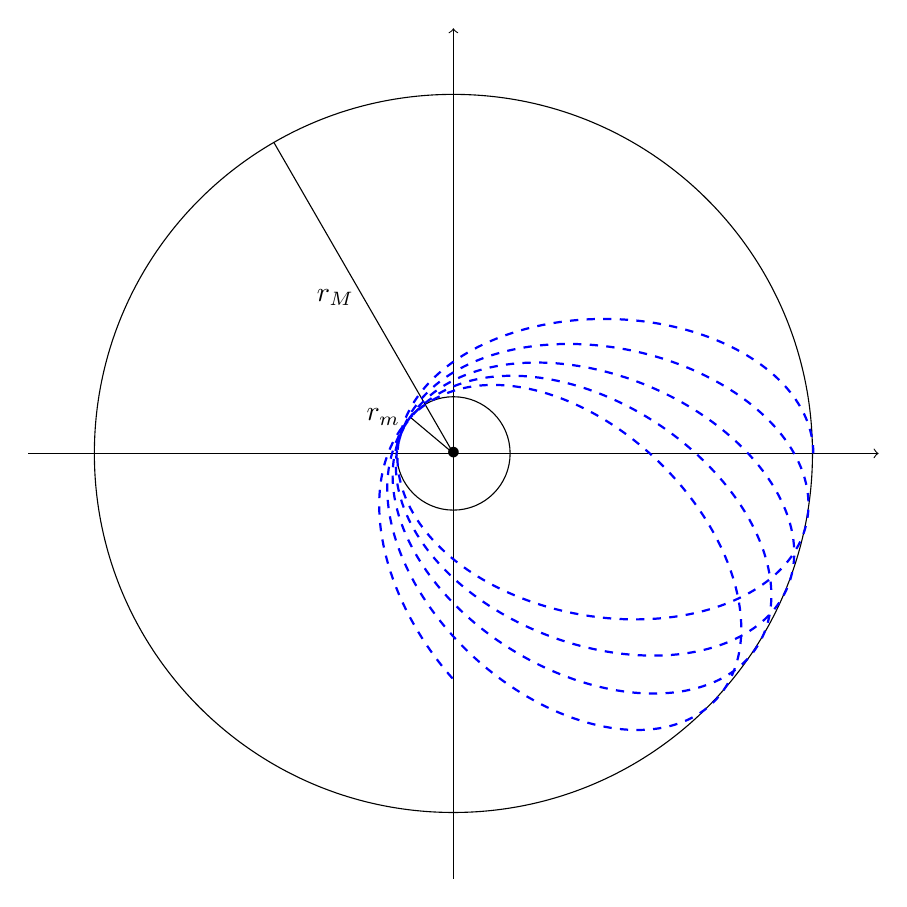
\begin{tikzpicture}[scale = 1.2]
                            \draw[->] (-4.5,0) -- (4.5,0);
                            \draw[->] (0,-4.5) -- (0,4.5);
                            \draw (0,0) circle (3.8);
                            \draw (0,0) circle (0.6);
                            \draw (0,0) node{$\bullet$};
                            %\draw[fill = black] (0,0) circle (0.3);
                            % X(t) = a*cos(t)+sqrt(a^2-b^2)
                            % Y(t) = b*sin(t)
                            \draw (0,0) -- (120:3.8) node[midway,left]{$r_M$};
                            \draw (0,0) -- (140:0.6) node[left]{$r_m$};
                            \draw[blue, dashed, thick, samples = 1000, domain=0:30] plot ({cos(deg(0.03*\x))*(2.2*cos(deg(\x))+1.6093)+sin(deg(0.03*\x))*(1.5*sin(deg(\x)))}, {-sin(deg(0.03*\x))*(2.2*cos(deg(\x))+1.6093)+cos(deg(0.03*\x))*(1.5*sin(deg(\x)))});
                        \end{tikzpicture}
                        \caption{Avancée du périastre}
                    \end{figure}
                    
                    on peut montrer que cette avancée est donnée par
                    \begin{equation}
                        \Delta \phi = \frac{6\pi GM}{ac^2(1-e^2)}
                    \end{equation}
                    
                    Le calcul de ce résultat est le sujet de la prochaine section.
                    
                    %schéma eliott
                    
                    Comme le potentiel possède deux maximas, deux trajectoire circulaire sont possibles. Cependant, un seule correspond à un minimum et donc une seul des deux trajectoire est stable (comme dans le cas newtonnien). Le rayon minimal d'une trajectoire circulaire stable est
                    \begin{equation}
                        R = \frac{6GM}{c^2}.
                    \end{equation}
                    En effet,
                    \comp
                    
                    On peut également montrer que le périastre minimal pour une trajectoire bornée est
                    \begin{equation}
                        r_m = \frac{4GM}{c^2}.
                    \end{equation}
                    Effectivement,
                    \comp
                    
                    \item $\bm{\mathscr{E}>0}$ : on a une trajectoire de type hyperbolique 
                \end{itemize}
                \item $\bm{12\left( \frac{GM}{c^2} \right)^2<L^2<16\left( \frac{GM}{c^2} \right)^2}$ : les trajectoires sont les même que précédemment mais il en existe certaine qui n'ont pas de $r_m$ (crash dans l'astre central).
                
                %schéma eliott
                
                On peut montrer que, si un particule arrive de l'infini avec une vitesse $\vv{v}$, alors elle est automatiquement happée par l'étoile si sont paramètre d'impact $a$ est tel que
                \begin{equation}
                    \frac{v}{c} <\frac{4GM}{ac^2}.
                \end{equation}
                
                \comp
                
                \item $\bm{L^2<12\left( \frac{GM}{c^2} \right)^2}$ : 
                
                %schéma eliott
                
            \end{itemize}
    
    \section{Calcul de l'avancée du périastre}
    
        Pour rappel, l'énergie
        \begin{equation}
            \mathscr{E} = \frac{1}{2}\dot{r}^2+V_{\text{eff}}(r)
        \end{equation}
        avec
        \begin{equation}
            V_{\text{eff}}(r) = \frac{1}{2}\left( 1-\frac{M}{r} \right)\frac{L^2}{r^2}-\frac{M}{r}
        \end{equation}
        est une constante du mouvement. Calculons l'évolution de l'angle $\phi$ après une période complète du mouvement radial. On peut déjà s'attendre à ce que $\Delta\phi = 2\pi$ dans le cas newtonien et $\Delta\phi>2\pi$ dans le cas de la relativité générale.\\
        
        Nous savons que, 
        \begin{equation}
            \frac{d\phi}{dr} = \frac{L}{r^2}
        \end{equation}
        ce qui permet d'exprimer $\Delta\phi$ comme
        \begin{equation}
            \Delta\phi = \int_{\text{1 période}}\frac{d\phi}{dr} = L\int_{\text{1 période}}\frac{d\tau}{r^2}.
        \end{equation}
        En utilisant l'expression de $\mathscr{E}$, on voit que
        \begin{align}
            \left( \frac{r}{\tau} \right)^2 &= 2(\mathscr{E}-V_{\text{eff}}(r))\\
            \Leftrightarrow\qquad dr &= \pm\sqrt{2\mathscr{E}-V_{\text{eff}}(r)}d\tau
        \end{align}
        et donc
        \begin{equation}
            \Delta\phi = L\int_{\text{1 période}}\frac{dr}{r^2\sqrt{2\mathscr{E}-V_{\text{eff}}(r)}} = 2L\int_{r_m}^{r_M}\frac{dr}{r^2\sqrt{2\mathscr{E}-V_{\text{eff}}(r)}}
        \end{equation}
        où $r_m$ et $r_M$ sont respectivement le périastre et l'apoastre, c'est-à-dire les racines positives de l'équation $V_{\text{eff}}(r)=\mathscr{E}$. Pour simplifier les calculs, posons $\rho=\frac{1}{r}$. Dans ce cas, $\frac{dr}{r^2} = -d\rho$ et 
        \begin{equation}
            \mathscr{E}-V_{\text{eff}}(r) = \underbrace{\mathscr{E}-\frac{1}{2}L^2\rho^2+M\rho}_{\text{Newton}}+\underbrace{\frac{1}{2}ML^2\rho^3}_{\text{perturbation}}.
        \end{equation}
        Notre stratégie pour aborder ce problème sera de considérer la terme en $\rho^3$ comme une petite perturbation au terme présent en mécanique newtonienne. Si l'on note
        \begin{align}
            \rho^{(0)}_M &\equiv \frac{1}{r^{(0)}_m}\\
            \rho^{(0)}_m &\equiv \frac{1}{r^{(0)}_M}
        \end{align}
        où $r^{(0)}_m$ et $r^{(0)}_M$ désignent respectivement le périastre et l'apoastre newtonniens, on peut réécrire
        \begin{equation}
            \mathscr{E}-V_{\text{eff}}(r) = \frac{1}{2}L^2\left( \rho-\rho^{(0)_m} \right)\left( \rho^{(0)_M}-\rho \right)+2M\rho^3.
        \end{equation}
        On obtient finalement l'intégrale suivante.
        \begin{equation}
            \Delta\phi = 2\int^{\rho_M}_{\rho_m}\frac{d\rho}{\sqrt{\left( \rho-\rho^{(0)}_m \right)\left( \rho^{(0)}_M-\rho \right)+2M\rho^3}}
        \end{equation}
        
        \subsection{Cas de Newton}
        
            Dans le cas newtonnien, le terme perturbatif est nul. L'intégrale est donc al suivante :
            \begin{equation}
                \Delta\phi = 2\int^{\rho_M}_{\rho_m}\frac{d\rho}{\sqrt{\left( \rho-\rho^{(0)}_m \right)\left( \rho^{(0)}_M-\rho \right)}}.
            \end{equation}
            Cet intégrale est bien convergente et peut être effectuée par calcul direct. Cependant, utilisons une autre approche qui, bien que plus compliquée dans ce cas-ci, pourra être ré-utilisée dans le cas de la relativité générale.\\
            
            La stratégie est de résoudre l'intégrale en utilisant le théorème des résidus sur l'intégrale complexe. Pour rappel, la fonction racine carrée est définie en analyse complexe comme
            \begin{equation}
                \sqrt{z}~\hat{=}~\sqrt{\abs{z}}~e^{\frac{i}{2}\arg(z)}
            \end{equation}
            pour tout $ł\in\mathbb{C}$ où $\arg(z)$ est la \textit{fonction argument} de $z$. L'important est que $(\sqrt{z})^2$ mais la fonction de l'argument peut être définie de différente manière. La détermination de l'argument la plus courante est d'utiliser l'angle polaire $\theta$:
            \begin{equation}
                \arg(z) = \theta = \arctan\left(\frac{\Im(z)}{\Re(z)}\right).
            \end{equation}
            c'est la \textit{détermination principale}. Cette détermination n'est pas continue. En effet, 
            \begin{equation}
                \lim\limits_{y\to0^+} \arg(x+iy) = 0 \neq 2\pi = \lim\limits_{y\to0^-} \arg(x+iy).
            \end{equation}
            La fonction argument n'est pas continue le long de la demi-droite $[0,+\infty]$ (coupure). On peut utiliser d'autre détermination de l'argument de manière à déplacer et à changer la forme de cette coupure à volonté mais il n'est pas possible de ne plus en avoir. En translatant la détermination principale, on peut par exemple faire en sorte que la coupure soit $[-\infty,0]$. Nous prendrons ces cas pour la suite.
            
            %schéma eliott
            
            Revenons à la fonction racine. A cause de la discontinuité de l'argument, la fonction racine est également discontinue le long de la même coupure. Pour voir cela, prenons $z_1,z_2\in\mathbb{C}$ de sorte que $z_1$ soit au dessus de la coupure et que $z_2$ soit en dessous de la coupure. Dans cas,
            \begin{align}
                \sqrt{z_1} &= i\sqrt{\abs{z_1}}\\
                \sqrt{z_2} &= -i\sqrt{\abs{z_2}}
            \end{align}
            Il y a donc une discontinuité de signe. Dans le cas de la racine de deux nombres complexe, on a 
            \begin{equation}
                \sqrt{(z-a)(z-b)} = \sqrt{\abs{z-a}\cdot\sqrt{\abs{z-b}}}e^{\frac{i}{2}\left( \arg(z-a)-\arg(z-b) \right)}
            \end{equation}
            avec $a,b\in\mathbb{R}$ et $a<b$. Il y a donc une coupure sur $[-\infty,a]$ (provenant de la fonction $\arg(z-a)$) et une coupure sur $[-\infty,b]$ (provenant de $\arg(z-b)$). Sur la demi-droite $\{x\in\mathbb{R}|x<a\}$ il y deux discontinuités de signe et donc l'effet s'annule. La coupure restante est sur l'intervalle $[a,b]$.\\
            
            Considérons la fonction
            \begin{equation*}
                z\mapsto \frac{1}{\sqrt{\left( z-a \right)\left( z-b \right)}}.
            \end{equation*}
            Cette fonction possède deux pôle et une coupure sur $[a,b]$. Si l'on intègre cette fonction sur un chemin fermé $\gamma_1$ qui entoure la coupure, alors l'intégrale peut se diviser en deux intégrales réelles où seul le signe de l'intégrant et le sens des bornes de l'intégrale change.
            \begin{align}
                \oint_{\gamma_1}\frac{dz}{\sqrt{\left( z-a \right)\left( z-b \right)}} &= \int_a^b \frac{dx}{(-i)\sqrt{\left( x-a \right)\left( x-b \right)}}+\int_b^a -\frac{dx}{(-i)\sqrt{\left( x-a \right)\left( x-b \right)}}\\
                &= 2i\int_a^b \frac{dx}{\sqrt{\left( x-a \right)\left( x-b \right)}}\\
                &= 2\pi i
            \end{align}
            par le théorème des résidus. Le facteur $-i$ vient de la racine complexe.\\
            
            Le théorème des résidus également affirme que cette intégrale est indépendante du chemin choisit. Prenons un second chemin $\gamma_{2,R}(t) = Re^{it}$, le cercle de rayon $R>\max(a,b)$. Dans ce cas
            \begin{equation}
                \lim\limits_{R\to\infty} \oint_{\gamma_{2,R}}\frac{dz}{\sqrt{\left( z-a \right)\left( z-b \right)}} = \lim\limits_{R\to\infty}\oint_{\gamma_{2,R}}\frac{dz}{z} = 2\pi.
            \end{equation}
            
            Dans le cas de notre intégrale, $a = \rho^{(0)}_m$ et $b = \rho^{(0)}_M$. Nous obtenons alors
            \begin{align}
                \oint_{\gamma_1} \frac{1}{\sqrt{\left( z-\rho^{(0)}_m \right)\left( \rho^{(0)}_M-z \right)}}~\frac{dz}{2\pi} &= \frac{1}{2\pi i} \int^{\rho_M}_{\rho_m}\frac{1}{-i\sqrt{\left( z-\rho^{(0)}_m \right)\left( \rho^{(0)}_M-z \right)}}~dz\\
                &= \frac{1}{\pi} \int^{\rho_M}_{\rho_m}\frac{d\rho}{\sqrt{\left( \rho-\rho^{(0)}_m \right)\left( \rho^{(0)}_M-\rho \right)}}
            \end{align}
            et
            \begin{equation}
                \oint_{\gamma_2} \frac{1}{\sqrt{\left( z-\rho^{(0)}_m \right)\left( \rho^{(0)}_M-z \right)}}~\frac{dz}{2\pi} = \oint_{\gamma_2}\frac{1}{z}~\frac{dz}{2\pi} = 1.
            \end{equation}
            Or, la valeur de l'intégrale ne doit pas dépendre du chemin. Ceci permet de conclure que
            \begin{equation}
                \frac{1}{\pi} \int^{\rho_M}_{\rho_m}\frac{d\rho}{\sqrt{\left( \rho-\rho^{(0)}_m \right)\left( \rho^{(0)}_M-\rho \right)}} = 1
            \end{equation}
            et donc que
            \begin{equation}
                \Delta\phi = 2 \frac{1}{\pi} \int^{\rho_M}_{\rho_m}\frac{d\rho}{\sqrt{\left( \rho-\rho^{(0)}_m \right)\left( \rho^{(0)}_M-\rho \right)}} = 2\pi.
            \end{equation}
        
        \subsection{Cas d'Einstein}
        
            Traitons le terme $M\rho^3$ perturbativement. C'est-à-dire que l'on peut se limiter au développement au premier ordre. Pour rappel, si $\varepsilon\ll1$,
            \begin{equation}
                \frac{1}{\sqrt{1+\varepsilon}}\approx1-\frac{\varepsilon}{2}
            \end{equation}
            et donc
            \begin{align}
                \Delta\phi &= 2\int^{\rho_M}_{\rho_m}\frac{d\rho}{\sqrt{\left( \rho-\rho^{(0)}_m \right)\left( \rho^{(0)}_M-\rho \right)+2M\rho^3}}\\
                &= 2\int^{\rho_M}_{\rho_m}\frac{d\rho}{\sqrt{\left( \rho-\rho^{(0)}_m \right)\left( \rho^{(0)}_M-\rho \right)}\left( 1+\frac{2M\rho^3}{\left( \rho-\rho^{(0)}_m \right)\left( \rho^{(0)}_M-\rho \right)} \right)^{\frac{1}{2}}} \\
                &\approx 2\pi + 2\int^{\rho^{(0)}_M}_{\rho^{(0)}_m}\frac{1}{\sqrt{\left( \rho-\rho^{(0)}_m \right)\left( \rho^{(0)}_M-\rho \right)}}\frac{M\rho^2}{\left( \rho-\rho^{(0)}_m \right)\left( \rho^{(0)}_M-\rho \right)} ~d\rho
            \end{align}
            Nous obtenons une intégrale divergente. Pour résoudre cette difficulté, on écrit
            \begin{align}
                \Delta\phi &= \frac{2}{2i}\oint_{\gamma_1}\frac{dz}{\sqrt{\left( z-\rho^{(0)}_m \right)\left( z-\rho^{(0)}_M \right)}-Mz^3}\\
                &\approx 2\phi+\frac{1}{i}\frac{2}{2i}\oint_{\gamma_1}\frac{1}{\sqrt{\left( z-\rho^{(0)}_m \right)\left( z-\rho^{(0)}_M \right)}}\frac{Mz^3}{2\left( z-\rho^{(0)}_m \right)\left( z-\rho^{(0)}_M \right)}~dz\\
                &= 2\pi-\frac{i}{2}\oint_{\gamma_1}\frac{Mz^3}{\left(\left( z-\rho^{(0)}_m \right)\left( z-\rho^{(0)}_M \right)\right)^{\frac{3}{2}}}~dz
            \end{align}
            pour un chemin $\gamma_1$ contour de la coupure. Comme pour le cas newtonnien, on peu prendre un second chemin $\gamma_2$ partant à l'infini pour lequel
            \begin{equation}
                \frac{1}{\left(\left( 1-\frac{\rho^{(0)}_m}{z} \right)\left( 1-\frac{\rho^{(0)}_M}{z} \right)\right)^{\frac{3}{2}}} = 1+\frac{1}{z}(\rho^{(0)}_m+\rho^{(0)}_M)^{\frac{3}{2}}+\dots
            \end{equation}
            En égalant les deux résultats, nous obtenons
            \begin{align}
                \Delta\phi &= 2\pi-\frac{2iM}{2}(2i\pi)\frac{3}{2}(\rho^{(0)}_m+\rho^{(0)}_M)^{\frac{3}{2}}\\
                &= 2\pi+3\pi M\left( \frac{1}{r^{(0)}_m}+\frac{1}{r^{(0)}_M} \right)
            \end{align}
            Or, pour rappel,
            \begin{equation}
                r = \frac{a(1-e^2)}{1-e\cos\theta}
            \end{equation}
            donc
            \begin{align}
                r_m &= \frac{a(1-e^2)}{1+e} = a(1-e)\\
                r_M &= \frac{a(1-e^2)}{1-e} = a(1+e)
            \end{align}
            En utilisant ces expressions, on trouve que
            \begin{equation}
                \frac{1}{r^{(0)}_m}+\frac{1}{r^{(0)}_M} = \frac{1}{a}\left( \frac{1}{1+e}+\frac{1}{1-e} \right) = \frac{2}{a(1-e^2)}
            \end{equation}
            ce qui permet de réécrire l'avance du périastre comme
            \begin{equation}
                \boxed{\Delta\phi = 2\pi+\frac{6\pi GM}{ac^2(1-e^2)}}
            \end{equation}
            
        \subsection{Applications numériques}
                
            Le phénomène d'avancée du périastre prédit par la relativité générale a permis d'expliquer l'avancée du périhélie de Mercure qui, observé depuis longtemps, n'avait jamais pu être réellement expliqué. L'avancée prédite par la théorie correspond exactement à ce qui est observé. Ceci a joué un grand rôle dans l'acceptation de cette théorie dans la communauté scientifique. Dans le cas de mercure,
            \begin{align}
                a &= 57.91\cdot10^8\meter\\
                e &= 0.2056\\
                \frac{GM_{\oplus}}{c^2} &= 1.475\kilo\meter
            \end{align}
            donc, si $\Delta\phi = 2\pi+(\Delta\phi)_{\text{Einstein}}$, on trouve
            \begin{equation}
                (\Delta\phi)_{\text{Einstein}} = 0.104''/\text{tour} = 43''/\text{siècle}.
            \end{equation}
            En réalité, la non-sphéricité du soleil joue également un rôle important dans l'avance du périhélie de Mercure ($\sim 532''/\text{siècle}$) mais cet effet avait déjà pu être calculé en mécanique newtonienne.\\
            
            Un autre astre a joué un rôle important lors de la validation de la théorie : la pulsar relativiste PSR 1913+16 constitué de deux étoiles à neutrons. Dans cas-ci,
            \begin{align}
                R &= 20\kilo\meter\\
                M_1 &\approx M_2 \approx 1.4M_{\odot}\\
                T &= 7.75\text{ heures}\\
                e &= 0.62
            \end{align}
            donc
            \begin{equation}
                (\Delta\phi)_{\text{Einstein}} = 6.3\cdot10^{-5}\radian/\text{révolution} = 0.071~\radian/\text{an}.
            \end{equation}
            
    \section{Déformation du temps}
    
        Dans cette partie, nous calculerons la déformation du temps subit par une horloge atomique embarquée dans un satellite. Supposons que la trajectoire est parfaitement circulaire.\\
        
        En relativité restreinte, le temps propre de l'horloge $\tau_h$ et le temps propre sur Terre $\tau_{\text{Terre}}$ sont reliés par
        \begin{equation}
            d\tau_h = \sqrt{1-v^2}~d\tau_{\text{Terre}} < d\tau_{\text{Terre}}
        \end{equation}
        où $v$ est la vitesse du satellite. L'horloge embarque retarde par rapport à l'horloge terrestre (dilatation du temps).\\
        
        Considérons maintenant le cas avec un champ de gravitation décrit par la métrique de Schwarzschild.
        
        \begin{prop}[troisième loi de Kepler]\begin{leftbar}
            Pour une trajectoire circulaire, 
            \begin{equation}
                \frac{r^3}{T^2_S} = \frac{M}{4\pi^2}
            \end{equation}
            où $T_S$ est la période de révolution dans les coordonnées de Schwarzschild.
        \end{leftbar}\end{prop}
        
        \begin{proof}
            Pour une trajectoire circulaire : $r_m=r_M$. Le rayon est donc donné par $V_{\text{eff}}'(r) = 0$.
            \begin{align}
                V_{\text{eff}}'(r) &= 0\\
                \Leftrightarrow\qquad -\frac{L^2}{r^3}+\frac{3ML^2}{r^4}+\frac{M}{r^2} &= 0\\
                \Leftrightarrow\qquad \frac{1}{r^3}\left( -L^2\left( 1-\frac{3M}{r}\right)+Mr \right) &= 0 \\
                \Leftrightarrow\qquad L^2 = \frac{Mr}{1-\frac{3M}{r}}\label{eq:L}
            \end{align}
            De plus, 
            \begin{equation}
                \frac{d\phi}{dt} = \frac{d\phi}{d\tau}\frac{d\tau}{dt} = \frac{\dot{\phi}}{\dot{t}} = \frac{L}{r^2}\frac{1}{\dot{t}}.
            \end{equation}
            Pour une trajectoire circulaire et la métrique de Schwarzschild, nous avons
            \begin{equation}
                d\tau^2 = \left( 1-\frac{2M}{r} \right)dt^2-r^2 d\phi^2.
            \end{equation}
            En utilisant la relation précédente, 
            \begin{alignat}{3}
                && d\tau^2 &= \left( 1-\frac{2M}{r} \right)dt^2-r^2 d\phi^2\\
                \Leftrightarrow&& \left(\frac{d\tau}{dt}\right)^2 &= \left( 1-\frac{2M}{r} \right)dt^2-r^2 \left(\frac{d\phi}{dt}\right)^2 \\
                \Leftrightarrow&& \frac{1}{\dot{t}^2} &= \left( 1-\frac{2M}{r} \right)-r^2\left(\frac{d\phi}{dt}\right)^2\\
                \Leftrightarrow&& \frac{r^4}{L^2}\left(\frac{d\phi}{dt}\right)^2 &= \left( 1-\frac{2M}{r} \right)-r^2\left(\frac{d\phi}{dt}\right)^2\\
                \Leftrightarrow&&~~ \left( \frac{r^4}{L^2} + r^2 \right)\left(\frac{d\phi}{dt}\right)^2 &= \left( 1-\frac{2M}{r} \right)\\
                \Leftrightarrow&& \left(\frac{d\phi}{dt}\right)^2 &= \left( 1-\frac{2M}{r} \right) \left( \frac{r^4}{L^2} + r^2 \right)^{-1}\label{eq:findevphit}
            \end{alignat}
            D'après la relation \ref{eq:L}, 
            \begin{equation}
                \frac{r^4}{L^2}+r^2 = \frac{r^4}{Mr}\left( 1-\frac{3M}{r} \right)+r^2 = \frac{r^3}{M}\left( 1-\frac{2M}{r} \right).
            \end{equation}
            En substituant dans l'équation \ref{eq:findevphit}, nous trouvons 
            \begin{equation}
                \left(\frac{d\phi}{dt}\right)^2 = \frac{1-\frac{2M}{r}}{1-\frac{2M}{r}}\frac{M}{r^3} = \frac{M}{r^3}
            \end{equation}
            donc
            \begin{equation}
                \frac{d\phi}{dt} = \frac{M}{r^{\frac{3}{2}}}.
            \end{equation}
            C'est la même relation qu'en mécanique newtonienne. On peut alors intégrer de $a$ à $T_S$, où $T_S$ est la période de révolution dans le temps de Schwarzschild (différent du temps physique).
            \begin{align}
                \int_0^{T_S}\frac{d\phi}{dt}~dt &= \int_0^{T_S}\frac{M}{r^{\frac{3}{2}}}~dt \\
                \Leftrightarrow\qquad 2\pi &= \frac{M}{r^{\frac{3}{2}}}T_S
            \end{align}
        \end{proof}
        
        La relation entre le temps propre $\tau_E$ d'un émetteur en orbite et la temps propre du récepteur $\tau_R$ sur la Terre est donnée par
        \begin{equation}
            d\tau^2_E = \left( 1-\frac{2M}{R} \right)~dt^2_E-R^2~d\phi^2
        \end{equation}
        en négligeant la rotation de la Terre. En utilisant la relation
        \begin{equation}
            d\phi^2 = \frac{M}{R^3}~dt^2_E
        \end{equation}
        qui a été utilisée dans la démonstration de la troisième loi de Kepler, nous pouvons reformuler $d\tau_E$ comme
        \begin{align}
            d\tau^2_E &= \left( 1-\frac{2M}{R}-R^2\frac{M}{R^3} \right)~dt^2_E\\
            &= \left( 1-\frac{3M}{R} \right)~dt^2_E
        \end{align}
        Par définition de $\tau_R$, 
        \begin{equation}
            d\tau^2_R = \left( 1-\frac{2M}{R_\oplus} \right)~dt^2_R.
        \end{equation}
        Lorsque le champ de gravitation est statique (c'est notre cas) donc $dt_E = dt_R$. En utilisant les deux relations précédentes, on trouve donc que
        \begin{equation}
            d\tau^2_R = \left( 1-\frac{2M}{R_\oplus} \right)~dt^2_E = \frac{1-\frac{2M}{R_\oplus}}{1-\frac{3M}{R}}~d\tau^2_E
        \end{equation}
        ou encore
        \begin{equation}
            d\tau_R = \sqrt{\frac{1-\frac{2M}{R_\oplus}}{1-\frac{3M}{R}}}~d\tau_E
        \end{equation}
        Le numérateur est d'origine gravitationnelle tandis que le dénominateur proviens aussi de la relativité restreinte. On peut voir que, si l'on veut que $d\tau_E<d\tau_R$ (comme la relativité restreinte le suggère), il faut que
        \begin{align}
            1-\frac{2M}{R_\oplus} &> 1-\frac{3M}{R} \\
            \Leftrightarrow\qquad \frac{3M}{R} &> \frac{2M}{R_\oplus}\\
            \Leftrightarrow \qquad R &< \frac{3}{2}R_\oplus
        \end{align}
        Dans ce cas, appelé \textit{orbite basse}, les de la relativité restreinte dominent. Au contraire, si
        \begin{equation}
            R > \frac{3}{2}R_\oplus
        \end{equation}
        dans le cas d'un\textit{orbite haute}, ce sont les effets de la relativité générale qui dominent : $$d\tau_E>d\tau_R$$. Ce résultat est à comparer avec le décalage des fréquences que nous avons discuté plus tôt (l'effet du décalage vers le bleu du au champ de gravitation l'emporte, donc l'horloge embarquée avance).\\
        
        Les ordres de grandeur typiques des effets du champ de gravitation sur le temps sont $\sim10^{-9}$. Ceci est particulièrement important pour le système de GPS par exemple. Pour repérer la position d'un émetteur sur la Terre, plusieurs GPS mesurent la distance entre leur position et celle de l'émetteur. Si $\Delta x$ est la résolution spatiale voulue sur Terre et que $L$ est une distance typique mesurée par le satellite, alors
        \begin{equation}
            \frac{\Delta x}{L}\sim\frac{2\centi\meter}{20~000\kilo\meter}\sim10^{-9}
        \end{equation}
        donc il faut tenir compte des effets du champ de gravitation. Sans cela, on ne pourrait pas atteindre de résolution inférieur à $\Delta x\sim100\meter$.
        
    \section{Trous noirs de Schwarzschild}
    
        \subsection{Introduction}
    
            On utilise les unités géométriques $G = c = 1$. Au début de ce chapitre, nous avons montré que si l'on impose la symétrique sphérique, la solution au équation d'Einstein dans le vide est la métrique de Schwarzschild
            \begin{equation}
                ds^2 = -\left( 1-\frac{2M}{r} \right)dt^2 + \left( 1-\frac{2M}{r} \right)^{-1}dr^2 + r^2d\Omega^2
            \end{equation}
            avec $d\Omega^2 = d\theta^2+\sin^2\theta d\phi^2$. Lorsque l'on considère une étoile de rayon $R$, cette métrique est bien définie dans le vide, c'est-à-dire lorsque $r>R$. Pour $r<R$, le tenseur énergie-impulsion n'est plus identiquement nul. Dans ce cas, il faudrait trouver le tenseur-impulsion qui décrit l'intérieur stellaire et résoudre à nouveau les équations d'Einstein dont le second membre est maintenant non-nul. Notons que la métrique ne dépend que de la masse $M$ de l'étoile et pas de son rayon $R$. En particulier, la métrique ne dépend pas de la densité l'étoile. Cependant, on voit que la métrique diverge lorsque $r\to2M$ donc que se passe-t-il si $R$ est assez petit pour permettre $r\leq2M$ ? 
            \begin{definition}
                Le rayon de Schwarszchild est défini comme  
                \begin{equation}
                    R_S =\frac{2GM}{c^2}.
                \end{equation}
            \end{definition}
            Dans un premier temps, on pourrait être tenter de dire que la métrique de Schwarzschild n'est définie que pour les étoiles dont le rayon est supérieur au rayon de Schwarzschild, c'est d'ailleurs le cas la plupart du temps (pour le soleil : $R_S\sim 1.5\kilo\meter$). Pour résumer :
            
            \begin{itemize}[label = \textbullet]
                \item $\bm{R>R_S}$ : lorsque $r>R$ la solution aux équations d'Einstein est la métrique de Schwarzschild et lorsque $r<R$ la métrique de Schwarzschild n'est plus valable car nous ne sommes plus dans le vide.
                \item $\bm{R<R_S}$ : lorsque $r>R_S$ la métrique de Schwarzschild semble bien définie mais diverge lorsque $r\to R_S$. Lorsque $R<r<R_S$, la métrique de Schwarzschild semble non-définie (non-physique) même si l'on se trouve quand même dans le vide. Lorsque $r<R$ la métrique de Schwarzschild n'est plus valable car nous ne somme plus dans le vide. Nous verrons que si $R<R_S$ alors l'étoile s'effondre et donc la métrique de Schwarzschild est définie dans toute la région $r<R_S$.
                \comp
            \end{itemize}
            
            Prenons la solution de Schwarzschild au sérieux pour toutes les valeurs de $r$. On se heurte à deux problèmes : la métrique est singulière en $r=2M$ et en $r=0$. Pour comprendre, cartographies en utilisant des géodésiques radiales de genre lumière. Notons que l'on peut facilement se ramener au cas des géodésiques de genre temps à partir de l'étude des géodésiques de genre lumière et que la partie de la métrique qui nous intéresse est la partie radial car c'est elle qui diverge. Pour une géodésique radiale de genre lumière,
            \begin{equation}
                0 = \left( 1-\frac{2M}{r} \right)dt^2 - \left( 1-\frac{2M}{r} \right)^{-1}dr^2
            \end{equation}
            donc
            \begin{equation}
                 dt = \pm \left( 1-\frac{2M}{r}dt^2 \right)^{-1} dr = \pm \frac{r}{r-2M}~dr = \pm\left( 1+\frac{2M}{r-2M} \right)~dr.
            \end{equation}
            Le signe décide si la géodésique est entrante ($+$) ou sortante ($-$). Pour une géodésique radial, 
            \begin{equation}
                V_{\text{eff}}(r) = \frac{1}{2}\left( 1-\frac{2M}{r} \right)\frac{L^2}{r^2} = 
            \end{equation}
            et donc
            \begin{equation}
                \mathscr{E} = \frac{1}{2}\dot{r}^2.
            \end{equation}
            Il suit que $\dot{r}$ est une constante. En intégrant l'expression de $dt$ que nous avons trouvée ci-dessus, on obtient une expression explicite de $t$.
            \begin{equation}
                t = \pm\left( r+2M\ln\left( \frac{r-2M}{2M} \right) \right) +  \text{cste}
            \end{equation}
            
            \begin{figure}[H]
            \centering
            \begin{tikzpicture}[scale = 1.2]
                \begin{axis}[axis lines = left,xlabel = $\nicefrac{r}{R_S}$, ylabel = {$t$},xmin=0, xmax=8,ymin=0, ymax=6,xtick={0,1,...,8},ytick={0,1,...,6}]
                % entrantes
                \foreach \c in {0,1,...,15}
                   \addplot [domain=1:8, samples=100, color=blue,] {-\x-ln(\x-1)+\c};
                \foreach \c in {1,2,...,6}
                   \addplot [domain=0:1, samples=100, color=blue,] {\x+ln(1-\x)+\c};
                % sortantes
                \foreach \c in {-9,-8,...,6}
                   \addplot [domain=1:8, samples=100, color=blue,dashed] {x+ln(\x-1)+\c};
                \addplot [domain=0:1, samples=100, color=blue,dashed] {-\x-ln(1-\x)};
                \foreach \c in {0,1,...,5}
                   \addplot [domain=0:1, samples=100, color=blue,dashed] {-\x-ln(1-\x)+\c};
                \end{axis}
            \end{tikzpicture}
            \caption{Géodésiques radiales de genre lumière entrantes et sortantes}
            \end{figure}
             
            \begin{definition}
                On définit la \textit{coordonnée de la tortue} comme
                \begin{equation}
                    r_*(r) ~\hat{=}~ r+2M\ln\left( \frac{r-2M}{2M} \right).
                \end{equation}
            \end{definition}
             
            En terme de la coordonnée de la tortue, la coordonnée $t$ s'exprime comme
            \begin{equation}
                 t = \pm r_*(r) + \text{cste}
            \end{equation}
             avec le signe + pour une géodésique entrante et le signe - pour une géodésique sortante.
             
            \begin{definition}
                On définit les \textit{coordonnées de genre lumière}
                \begin{align}
                    t_1 ~&\hat{=}~ t+r_*(r)-r\\
                    u_1 ~&\hat{=}~ t_1+r
                \end{align}
                pour une géodésique entrante et
                \begin{align}
                    t_2 ~&\hat{=}~ t-r_*(r)-r\\
                    u_2 ~&\hat{=}~ t_2+r
                \end{align}
                pour une géodésique sortante.
            \end{definition}
            Notons que 
            \begin{align}
                u_1 &= t+r_*(r)\\
                u_2 &= t-r_*(t)
            \end{align}
            Donc $u_1=\text{cste}$ et $u_1=\text{cste}$.\\
            

            
            Dans un premier temps, étudier les géodésiques rentrantes. On peut voir que $t\to\infty$ lorsque $r\to 2M^+$ donc pour les observateurs qui restent à $r> 2M$, la géodésique entrante ne traverse jamais $r=2M$.
            
            \begin{definition}
                La sphère de rayon $r=2M$ est appellée \textit{horizon}.
            \end{definition}
            
            % schéma eliott
            
            De manière reliée, le décalage vers le rouge à l'horizon diverge. Notons que le champ de gravitation n'est pas forcément extrêmement fort à l'horizon. Du point de vue de l'observateur à l'extérieur, le temps écoulé pour se rapprocher de $r=2M$ est exponentiellement long. Pour l'observateur qui suit la géodésique entrante $\dot{r}$ est constant donc
            \begin{equation}
                r(\lambda) = -\lambda+\text{cste}.
            \end{equation}
            Il se voit atteindre et franchir $r=2M$ en un paramètre affinne fini (ou temps un temps fini dans le cas d'une géodésique de genre temps). Dans son référentiel, la géodésique croise l'horizon.\\
            
            Utilisons les coordonnées $t$ et $u_1$ qui sont mieux adaptée aux géodésiques entrantes. Par définition, 
            \begin{align}
                du_1 &= dt+dr_*\\
                &= dt + \left( 1+\frac{2M}{r-2M} \right)~dr\\
                &= dt +\frac{r}{2M}\frac{1}{\frac{r}{2M}-1}
            \end{align}
            donc la métrique se réécrit comme
            \begin{equation}
                ds^1 = -\left( 1-\frac{2M}{r} \right)~du^2_1 + 2du_1dr+r^2d\Omega^2
            \end{equation}
            Ces coordonnées montrent qu'il n'y a aucune singularité en $r=2M$ : ce sont uniquement les coordonnées de Schwarzschild qui sont singulière en $r=2M$. C'est une singularité apparente comme pour la singularité des coordonnées polaires dans le plan (l'angle polaire n'est pas définit lorsque le rayon est nul).\\
            
            % schéma eliott
            
            On peut diviser l'espace en deux régions :
            \begin{itemize}[label = \textbullet]
                \item \textbf{région I} $(\bm{r>2M})$ :  Cette région est asymptotiquement plate. Pour un observateur extérieur, les cônes de lumières se redressent du coté du trou noir au fur et à mesure que l'on s'en approche de manière à ce que les géodésiques ne pénètrent jamais l'horizon. Pour un observateur suivant une géodésique entrante, c'est le coté opposé du cône de lumière qui devient verticale en s'approchant de $r=2M$. Si l'on franchi l'horizon en venant de la région I, on pénètre dans la région $II$. 
                \item \textbf{région II} $(\bm{r<2M})$ : Une fois l'horizon passée, les cônes de lumière continuent à se refermer ce qui implique que toutes les trajectoires vont vers les $r$ décroissants.
            \end{itemize}
            Lorsque l'on dépasse l'horizon, les deux première composantes de ma métrique de Schwarzschild changent de signe donc $r$ de vient une coordonnée temporelle $t$ devient une coordonnée spatiale. Ceci implique que le champ de gravitation n'est pas statique quand $r<2M$, la métrique n'est plus invariante par rotation. La singularité $r=0$ est dans le futur de tout les observateurs. Il est faut de dire que l'on se fait attiré très fort par la gravité au point de ne plus pouvoir sortit; l'observateur va en fait simplement vers son futur. Ceci décrit une cosmologie de \textit{Big Crunch} à savoir une compression qui a lieu partout à la fois dans le futur. C'est l'inverse d'un \textit{Big Bang}, c'est-à-dire une explosion qui a lieu partout à la fois dans le passé. De cette manière, l'intérieur d'un trou noir de Schwarzschild décrit une cosmologie inversée pour laquelle le futur de tout les observateurs et dans la singularité en $r=0$. Notons que $r=0$ n'est pas une singularité apparente comme celle en $r=2M$ pour les coordonnées de Schwarzschild. Ceci peut être vu en observant que les invariants de courbure divergent : c'est une vraie singularité au-delà de laquelle les géodésiques ne peuvent pas êtres continuées. On dit que c'est un \textit{singularité de genre espace} car elle est partout dans l'espace en un point du temps.\\
            
            % schéma de eliott
            
            Étudions maintenant les géodésiques sortantes. Pour cela, on exprime la métrique dans la coordonnées $u_2$.
            \begin{align}
                ds^2 &= -\left( 1-\frac{2M}{r} \right)(dt^2-dr^2)+r^2 d\Omega^2\\
                &= -\left( 1-\frac{2M}{r} \right)(dt-dr)(dt+dr)+r^2 d\Omega^2\\
                &= -\left( 1-\frac{2M}{r} \right)du_1\left( du_1-2\frac{dr_*}{1-\frac{2M}{r}} \right)+r^2 d\Omega^2\\
                &= -\left( 1-\frac{2M}{r} \right)du^2_1+du_1dr+r^2 d\Omega^2\\
                &= -\left( 1-\frac{2M}{r} \right)du_2\left( du_2+2\frac{dr}{1-\frac{2M}{r}} \right)+r^2 d\Omega^2\\
                &= -\left( 1-\frac{2M}{r} \right)du^2_2-2du_2dr+r^2 d\Omega^2
            \end{align}
            
            On voit que les géodésiques sortantes qui sont dans la région II croisent l'horizon en un paramètre affinne dans le passé, c'est à nouveau un problème dû au coordonnées. Les géodésiques sortantes doivent sortir d'une région $r<2M$ mais ne peuvent pas sortir de la région II car, comme nous le verrons après, il n'y a pas de géodésiques sortantes de II). Les géodésiques sortante dans la région III proviennent donc d'une région III.\\
            
            Les géodésiques sortantes de la région II ne sortent jamais réellement. 
            Les géodésiques entrantes qui sont dans la région I ne peuvent pas venir de la région II, ce ne sont pas les mêmes que les géodésiques entrantes qui viennent de la région II. Elles viennent donc d'une région IV.\\
            
            % schéma eliott
            
            D'après ce que l'on vient de voir, les trous noir de Scwarzschild rejoignent deux régions de l'espace-temps séparée, la région I/II et la région III/IV. C'est un \textit{trou de ver}. A l'autre extrémité du trou de ver, la métrique est la même mais pas les cônes de lumière, tout les géodésiques sortent : c'est un \textit{trou blanc}. L'intérieur d'un trou décrit à une cosmologie de Big Bang (et plus de Big Crunch comme pour les trous noirs). 
            
            \begin{rmk}
                Si $R<2M$, il n'y a plus de solution statique pour le champ de gravitation, la surface de l'astre suit une géodésique de genre temps et l'astre s'effondre jusqu'à donner une singularité. Dans ce cas, il n'y a pas de région III et IV et donc pas de trou de ver.
                
                % schéma eliott
                
                Les trous noir dont on parle dan cette section sont considéré comme "éternels", on doit pouvoir remonter dans le passé aussi loin que l'on veut.
            \end{rmk}
            
            On a pu voir qu'il y a deux régions différentes telles que $r<2M$ et deux régions différentes telles que $r>2M$ donc la coordonnés radiale $r$ n'est pas une bonne coordonnée. On peut montrer que n'importe quel fonction des coordonnées $u_1$ et $u_2$ préserve les propriétés importantes de ces coordonnées. Définissons un nouveau type de coordonnées qui permet d'éliminer la singularité et donc de mieux représenter les trous de ver.
            
            \begin{definition}
                Les \textit{coordonnées de Kruskal-Szekeres} sont définies comme
                \begin{align}
                    U ~&\hat{=}~ e^{\frac{u_1}{4M}}\\
                    V ~&\hat{=}~ -e^{\frac{u_2}{4M}}
                \end{align}
            \end{definition}
            
            On peut directement voir que 
            \begin{align}
                UV &= -e^{\frac{u_1-u_2}{4M}} = -e^{\frac{r_*}{2M}}\frac{2M}{r}\frac{e^{-\frac{r}{2M}}}{1-\frac{2M}{r}}\\
                \frac{U}{V} &= -e^{\frac{u_1+u_2}{4M}} = -e^{\frac{t}{2M}}
            \end{align}
            
            et donc
            \begin{equation}
                dUdV = -\frac{du_1}{4M}\frac{du_2}{4M}UV = -\frac{du_1du_2}{32M^2}e^{-\frac{r}{2M}}\left( 1-\frac{2M}{r} \right)
            \end{equation}
            ce qui permet de réécrire la métrique dans les coordonnées de Krusal-Szekeres comme
            \begin{equation}
                ds^2 = 32M^2e^{-\frac{r}{2M}}dUdV+r^2d\Omega^2.
            \end{equation}
            Dans ces coordonnées, les lignes deviennt
            \begin{align}
                t &= \text{cste} \to \frac{U}{V} = \text{cste}\\
                r &= \text{cste} \to UV = \text{cste}
            \end{align}
            
            % schéma eliott
            
            \begin{figure}[H]
                \centering
                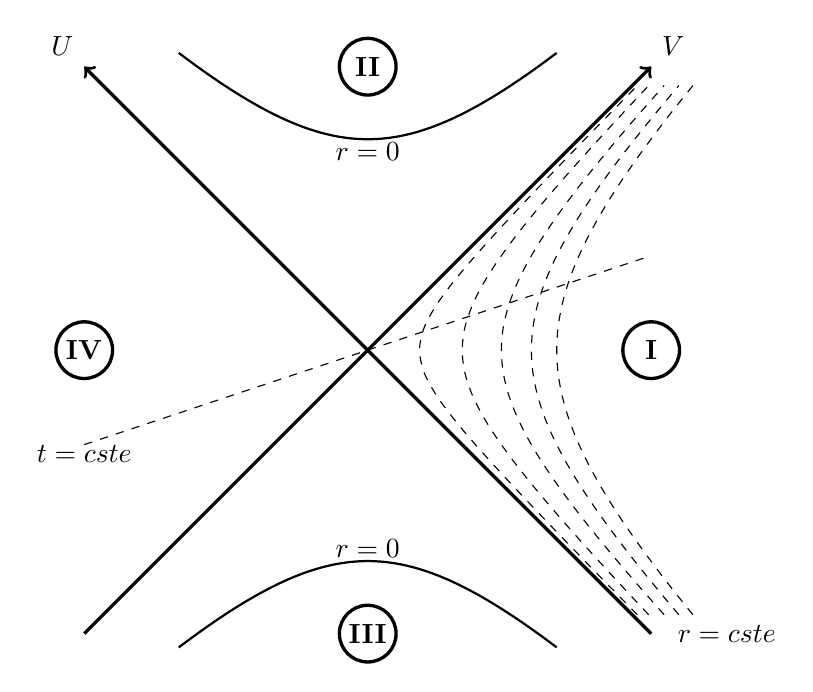
\begin{tikzpicture}[scale = 1.2]
                    \draw[->,very thick] (-3,-3) -- (3,3) node[above right]{$V$};
                    \draw[->,very thick] (3,-3) -- (-3,3) node[above left]{$U$};
                    \draw[domain=-2:2,smooth,variable=\x,thick] plot({\x},{sqrt(3+\x*\x))+0.5});
                    \draw (0,2.1) node{$r=0$};
                    \draw[domain=-2:2,smooth,variable=\x,thick] plot({\x},{-sqrt(3+\x*\x))-0.5});
                    \draw (0,-2.1) node{$r=0$};
                    
                    \draw (-3,0) node{\textbf{IV}};
                    \draw[very thick] (-3,0) circle (0.3);
                    \draw (3,0) node{\textbf{I}};
                    \draw[very thick] (3,0) circle (0.3);
                    \draw (0,-3) node{\textbf{III}};
                    \draw[very thick] (0,-3) circle (0.3);
                    \draw (0,3) node{\textbf{II}};
                    \draw[very thick] (0,3) circle (0.3);
                    
                    \draw[domain=-2.8:2.8,smooth,variable=\x,dashed] plot({sqrt(0.3+\x*\x))},{\x});
                    \draw[domain=-2.8:2.8,smooth,variable=\x,dashed] plot({sqrt(1+\x*\x))},{\x});
                    \draw[domain=-2.8:2.8,smooth,variable=\x,dashed] plot({sqrt(2+\x*\x))},{\x});
                    \draw[domain=-2.8:2.8,smooth,variable=\x,dashed] plot({sqrt(3+\x*\x))},{\x});
                    \draw[domain=-2.8:2.8,smooth,variable=\x,dashed] plot({sqrt(4+\x*\x))},{\x});
                    \draw (3.8,-3) node{$r=cste$};
                    
                    \draw[dashed] (-3,-1) -- (3,1);
                    \draw (-3,-1.1) node{$t=cste$};
                \end{tikzpicture}
                \caption{Diagramme de Kruskal-Szekeres}
            \end{figure}
            
        \subsection{Pont d'Einstein-Rosen}
        
            Si l'on décrit l'espace-temps au cours du temps, on voit que les deux régions de l'espace asymptotiquement plates déconnectée jusqu'à ce qu'au moment où le trou de ver s'ouvre, c'est le \textit{pont d'Einstein-Rosen}. A ce moment-là, les régions I et IV deviennent causalement connectées et un trou noir apparaît dans ces régions qui sont maintenant équivalentes (l'espace-temps devient connexe). Les régions II et III ne sont pas équivalentes (Big Bang ou Big Crunch). Ce type de trou de verre n'est pas traversable classiquement mais il existe d'autres types de trou de ver qui le sont.
        
        \subsection{Discussions plus avancées}